%-----------------------------------------------------------------------------%
\chapter{\babEmpat}
\label{chap:babEmpat}
%-----------------------------------------------------------------------------%

Pada bab ini dijelaskan hasil evaluasi dan analisis dari penelitian ini.

%-----------------------------------------------------------------------------%
\section{Evaluasi}
%-----------------------------------------------------------------------------%

Dua eksperimen pada penelitian ini dilakukan pada \textit{notebook} dengan sistem operasi \textit{Ubuntu 15.04 64-bit}, prosesor \textit{Intel Core i7 5500U} (\textit{dual cores}), RAM DDR3 8 GB dan penyimpanan SSD 250 GB. Program yang digunakan untuk melakukan eksperimen pertama adalah \verb|classifier.py| sedangkan eksperimen yang kedua menggunakan program \verb|extract_triples.py| (terlampir).

Pada eksperimen pertama, empat model \textit{supervised learning} dilatih dan diuji menggunakan data kandidat \textit{triple} yang sudah diberikan label, diekstraksi menjadi 17 fitur dan dinormalisasi. Metode yang digunakan untuk melatih dan menguji adalah \textit{k-fold} \textit{cross-validation} \citep{kohavi1995study} dengan variasi nilai $k = {2, 3, 5, 7, 10}$. Empat model yang dibandingkan beserta dengan konfigurasinya adalah sebagai berikut:

\begin{enumerate}

	\item Linear Logistic Regression
	\begin{itemize}
		\item Solver (cost function): \verb|liblinear|
		\item Penalty (regularizer): \verb|l2|
	\end{itemize}

	\item Polynomial Support Vector Machine (SVM)
	\begin{itemize}
		\item Kernel: \verb|poly|
		\item Degree: \verb|5|
	\end{itemize}

	\item ReLU Multi-Layer Perceptron (MLP)
	\begin{itemize}
		\item Hidden layers: \verb|(20, 10)|
		\item Activation: \verb|relu| \citep{nair2010rectified}
		\item Max. iteration: \verb|1000|
	\end{itemize}
	
	\item Random Forest
	\begin{itemize}
		\item Max. depth: \verb|8|
		\item Number of estimators: \verb|20|
		\item Min. samples split: \verb|5|
		\item Criterion: \verb|gini| \citep{mingers1989empirical}
		\item Max. features: \verb|auto| (pembulatan akar dari jumlah total fitur)
		\item Class weight: \verb|balanced| (sesuai rasio kelas)
	\end{itemize}

\end{enumerate}

Eksperimen ini dilakukan dengan menjalankan program \verb|classifier.py| (di direktori yang sama dengan pustaka utama \verb|tripletools.py|) dengan input \textit{dataset} fitur yang sudah dinormalisasi dengan format \textit{comma separated value} (CSV) \verb|triple-selector.train.csv| pada \textit{terminal}:

\begin{verbatim}
	$ python classifier.py --mode compare_models --cv 2 triple-selector.train.csv
	$ python classifier.py --mode compare_models --cv 3 triple-selector.train.csv
	$ python classifier.py --mode compare_models --cv 5 triple-selector.train.csv
	$ python classifier.py --mode compare_models --cv 7 triple-selector.train.csv
	$ python classifier.py --mode compare_models --cv 10 triple-selector.train.csv
\end{verbatim}

Hasil dari eksperimen pertama ini dapat dilihat pada Tabel \ref{tab:models_performance_k_2}, \ref{tab:models_performance_k_3}, \ref{tab:models_performance_k_5}, \ref{tab:models_performance_k_7} dan \ref{tab:models_performance_k_10}. Tetapi karena jika melihat standar deviasi yang terlalu tinggi (di atas 0.1) untuk $k > 3$ pada Tabel \ref{tab:models_performance_stdev} dan diagram Gambar \ref{fig:models_performance_stdev}, maka hasil yang kita amati adalah k-\textit{fold} \textit{cross-validation} dengan $k={2, 3}$ yang visualisasinya ditunjukkan pada Gambar \ref{fig:models_performance_k_2} dan Gambar \ref{fig:models_performance_k_3}. Dapat dilihat bahwa \textit{random forest} lebih tinggi dari model lainnya untuk $k=3$ dan sebanding dengan SVM untuk $k=2$. SVM hampir selalu mencapai nilai \textit{precision} tertinggi dalam semua eksperimen tetapi dengan nilai \textit{recall} yang lebih rendah dari model lain. Sedangkan \textit{random forest} bukan hanya mencapai nilai $F_1$ yang hampir selalu lebih tinggi, tapi juga memiliki nilai \textit{precision} dan \textit{recall} yang seimbang. 

\begin{table}
	\caption{Hasil k-\textit{fold} \textit{cross-validation} $k=2$ model \textit{supervised learning} untuk \textit{triple selector}}
	\label{tab:models_performance_k_2}
	\centering
	\begin{tabular}{p{5cm} >{\centering\arraybackslash}p{2cm} >{\centering\arraybackslash}p{2cm} >{\centering\arraybackslash}p{2cm}}
		\hline
		\textbf{Model} & \textbf{\textit{Precision}} & \textbf{\textit{Recall}} & \textbf{$F_1$} \\
		\hline
		Logistic Regression & 0.58 & 0.29 & 0.38 \\
		SVM & \textbf{0.70} & 0.39 & \textbf{0.50} \\
		MLP & 0.46 & 0.35 & 0.39 \\
		Random Forest & 0.52 & \textbf{0.49} & \textbf{0.50} \\
		\hline
	\end{tabular}
\end{table}

\begin{table}
\caption{Hasil k-\textit{fold} \textit{cross-validation} $k=3$ model \textit{supervised learning} untuk \textit{triple selector}}
	\label{tab:models_performance_k_3}
	\centering
	\begin{tabular}{p{5cm} >{\centering\arraybackslash}p{2cm} >{\centering\arraybackslash}p{2cm} >{\centering\arraybackslash}p{2cm}}
		\hline
		\textbf{Model} & \textbf{\textit{Precision}} & \textbf{\textit{Recall}} & \textbf{$F_1$} \\
		\hline
		Logistic Regression & 0.64 & 0.28 & 0.37 \\
		SVM & \textbf{0.69} & 0.42 & 0.51 \\
		MLP & 0.55 & 0.46 & 0.47 \\
		Random Forest & 0.62 & \textbf{0.58} & \textbf{0.58} \\
		\hline
	\end{tabular}
\end{table}

\begin{table}
	\caption{Hasil k-\textit{fold} \textit{cross-validation} $k=5$ model \textit{supervised learning} untuk \textit{triple selector}}
	\label{tab:models_performance_k_5}
	\centering
	\begin{tabular}{p{5cm} >{\centering\arraybackslash}p{2cm} >{\centering\arraybackslash}p{2cm} >{\centering\arraybackslash}p{2cm}}
		\hline
		\textbf{Model} & \textbf{\textit{Precision}} & \textbf{\textit{Recall}} & \textbf{$F_1$} \\
		\hline
		Logistic Regression & 0.69 & 0.26 & 0.36 \\
		SVM & \textbf{0.74} & 0.39 & \textbf{0.49} \\
		MLP & 0.54 & 0.39 & 0.41 \\
		Random Forest & 0.59 & \textbf{0.52} & \textbf{0.49} \\
		\hline
	\end{tabular}
\end{table}

\begin{table}
	\caption{Hasil k-\textit{fold} \textit{cross-validation} $k=7$ model \textit{supervised learning} untuk \textit{triple selector}}
	\label{tab:models_performance_k_7}
	\centering
	\begin{tabular}{p{5cm} >{\centering\arraybackslash}p{2cm} >{\centering\arraybackslash}p{2cm} >{\centering\arraybackslash}p{2cm}}
		\hline
		\textbf{Model} & \textbf{\textit{Precision}} & \textbf{\textit{Recall}} & \textbf{$F_1$} \\
		\hline
		Logistic Regression & 0.71 & 0.27 & 0.36 \\
		SVM & \textbf{0.69} & 0.38 & \textbf{0.47} \\
		MLP & 0.50 & 0.38 & 0.38 \\
		Random Forest & 0.52 & \textbf{0.49} & \textbf{0.47} \\
		\hline
	\end{tabular}
\end{table}

\begin{table}
	\caption{Hasil k-\textit{fold} \textit{cross-validation} $k=10$ model \textit{supervised learning} untuk \textit{triple selector}}
	\label{tab:models_performance_k_10}
	\centering
	\begin{tabular}{p{5cm} >{\centering\arraybackslash}p{2cm} >{\centering\arraybackslash}p{2cm} >{\centering\arraybackslash}p{2cm}}
		\hline
		\textbf{Model} & \textbf{\textit{Precision}} & \textbf{\textit{Recall}} & \textbf{$F_1$} \\
		\hline
		Logistic Regression & 0.70 & 0.26 & 0.36 \\
		SVM & \textbf{0.76} & 0.37 & 0.46 \\
		MLP & 0.59 & 0.36 & 0.40 \\
		Random Forest & 0.54 & \textbf{0.48} & \textbf{0.47} \\
		\hline
	\end{tabular}
\end{table}

\begin{table}
	\caption{Standar deviasi k-\textit{fold} \textit{cross-validation} $k={2, 3, 5, 7, 10}$ model \textit{supervised learning} untuk \textit{triple selector}}
	\label{tab:models_performance_stdev}
	\centering
	\begin{tabular}{l r r r r r}
		\hline
		\textbf{Model} & $k=2$ & $k=3$ & $k=5$ & $k=7$ & $k=10$ \\
		\hline
		Logistic Regression & 0.03 & 0.05 & 0.06 & 0.10 & 0.13 \\
		SVM & 0.03 & 0.05 & 0.06 & 0.10 & 0.13 \\
		MLP & 0.03 & 0.05 & 0.06 & 0.10 & 0.13 \\
		Random Forest & 0.04 & 0.09 & 0.12 & 0.13 & 0.23 \\
		\hline
	\end{tabular}
\end{table}

\begin{figure}
	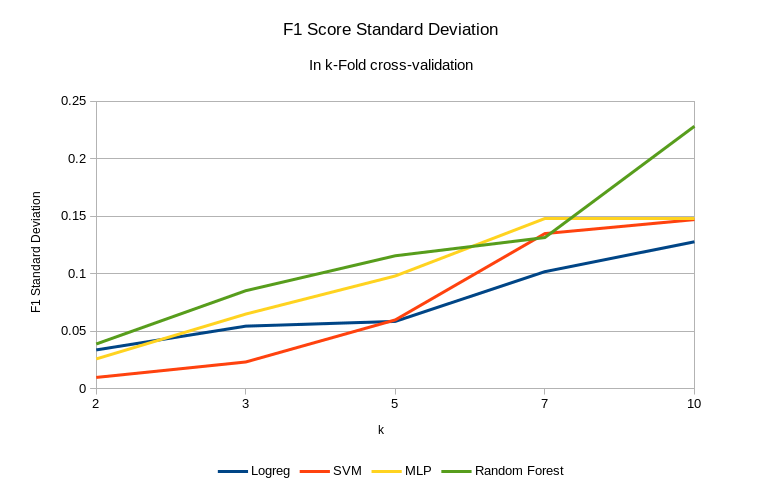
\includegraphics[width=\textwidth]{../images/models_performance_stdev.png}
	\caption{Diagram standar deviasi k-\textit{fold} \textit{cross-validation} $k={2, 3, 5, 7, 10}$ model \textit{supervised learning} untuk \textit{triple selector}}
	\label{fig:models_performance_stdev}
\end{figure}

\begin{figure}
	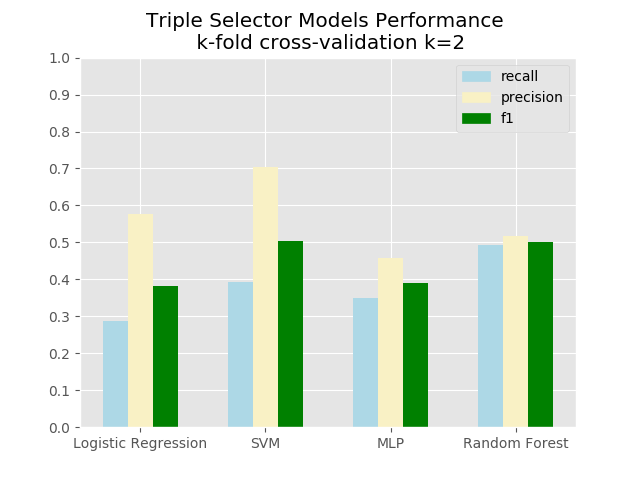
\includegraphics[width=\textwidth]{../images/models_performance_k_2.png}
	\caption{Diagram k-\textit{fold} \textit{cross-validation} model \textit{supervised learning} untuk \textit{triple selector} dengan $k=2$}
	\label{fig:models_performance_k_2}
\end{figure}

\begin{figure}
	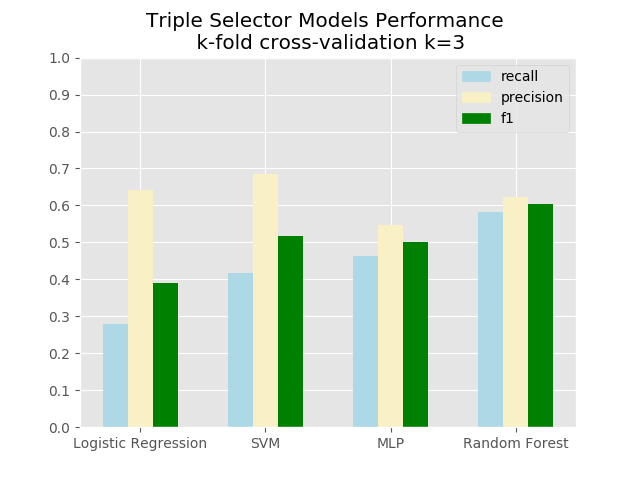
\includegraphics[width=\textwidth]{../images/models_performance_k_3.png}
	\caption{Diagram k-\textit{fold} \textit{cross-validation} model \textit{supervised learning} untuk \textit{triple selector} dengan $k=3$}
	\label{fig:models_performance_k_3}
\end{figure}


Pada eksperimen kedua, sistem \textit{open IE} dipakai untuk mengekstrak \textit{triple} dokumen dengan lima variasi ukuran/jumlah kalimat, yaitu 5, 10, 100, 1,000 dan 5,000 kalimat per dokumen. Untuk setiap variasi ukuran dokumen, digunakan 10 buah dokumen yang berbeda dengan ukuran yang identik sehingga total ada 50 dokumen berbeda yang digunakan dalam eksperimen ini. Kalimat-kalimat dalam dokumen uji ini diambil secara acak dari berbagai jenis artikel berita dan ensiklopedia bahasa Indonesia di internet sehingga dapat mewakili karakteristik \textit{open domain}.

Metrik pada eksperimen ini adalah waktu proses per kalimat (detik) dan jumlah \textit{triple} yang diekstraksi per kalimat. Eksperimen ini dilakukan dengan menjalankan program utama \verb|extract_triples.py| untuk setiap dokumen dengan format perintah:

\begin{verbatim}
	$ python extract_triples.py -f tsv doc.txt
\end{verbatim}

\begin{figure}
	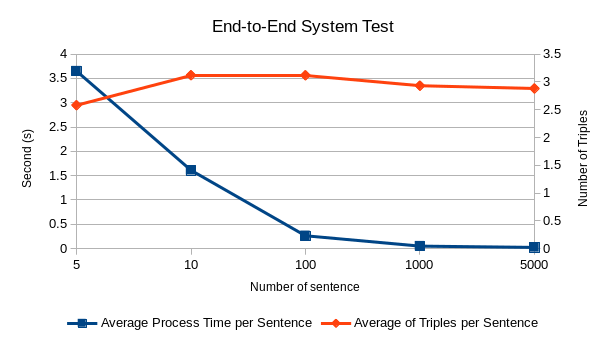
\includegraphics[width=\textwidth]{../images/system_performance.png}
	\caption{Rata-rata waktu proses per kalimat dan rata-rata jumlah \textit{triple} yang dihasilkan per kalimat pada variasi ukuran dokumen}
	\label{fig:system_performance}
\end{figure}

\begin{table}
	\caption{Waktu proses per kalimat (detik)}
	\label{tab:system_extraction_time}
	\centering
	\begin{tabular}{l *{5}{c}}
		\hline
		\textbf{No} & \multicolumn{5}{c}{\textbf{Ukuran Dokumen}} \\
		\cline{2-6}
		& \textbf{5} & \textbf{10} & \textbf{100} & \textbf{1,000} & \textbf{5,000} \\
		\hline			
		1 & 4.65 & 1.71 & 0.23 & 0.05 & 0.02 \\
		2 & 2.59 & 1.69 & 0.21 & 0.05 & 0.02 \\
		3 & 3.82 & 1.50 & 0.25 & 0.05 & 0.02 \\
		4 & 3.69 & 1.66 & 0.25 & 0.05 & 0.02 \\
		5 & 3.47 & 1.63 & 0.25 & 0.05 & 0.02 \\
		6 & 3.52 & 1.49 & 0.24 & 0.05 & 0.02 \\
		7 & 2.60 & 1.50 & 0.26 & 0.05 & 0.02 \\
		8 & 3.42 & 1.52 & 0.50 & 0.05 & 0.02 \\
		9 & 5.61 & 1.77 & 0.23 & 0.05 & 0.02 \\
		10 & 3.16 & 1.64 & 0.22 & 0.05 & 0.02 \\
		\hline
		\textbf{Rata-rata} & \textbf{3.65} & \textbf{1.61} & \textbf{0.26} & \textbf{0.05} & \textbf{0.02} \\
		\hline
	\end{tabular}
\end{table}

\begin{table}
	\caption{Jumlah \textit{triple} yang diekstraksi per kalimat}
	\label{tab:system_extraction_triple}
	\centering
	\begin{tabular}{l *{5}{c}}
		\hline
		\textbf{No} & \multicolumn{5}{c}{\textbf{Ukuran Dokumen}} \\
		\cline{2-6}
		& \textbf{5} & \textbf{10} & \textbf{100} & \textbf{1,000} & \textbf{5,000} \\
		\hline			
		1 & 1.80 & 1.90 & 3.25 & 2.98 & 2.88 \\
		2 & 1.80 & 3.00 & 3.43 & 2.95 & 2.74 \\
		3 & 1.60 & 3.20 & 2.97 & 2.74 & 2.86 \\
		4 & 2.40 & 3.70 & 3.16 & 3.00 & 2.95 \\
		5 & 1.00 & 4.00 & 3.02 & 3.04 & 2.93 \\
		6 & 2.40 & 4.30 & 3.62 & 2.80 & 2.80 \\
		7 & 2.20 & 3.70 & 2.96 & 2.94 & 2.87 \\
		8 & 3.20 & 1.30 & 3.13 & 2.92 & 3.00 \\
		9 & 4.80 & 3.00 & 3.09 & 2.98 & 2.91 \\
		10 & 4.60 & 3.10 & 2.56 & 2.98 & 2.89 \\
		\hline
		\textbf{Rata-rata} & \textbf{2.58} & \textbf{3.12} & \textbf{3.12} & \textbf{2.93} & \textbf{2.88} \\
		\hline
	\end{tabular}
\end{table}


Hasil eksperimen tersebut ditunjukkan pada Tabel \ref{tab:system_extraction_time} di mana waktu proses rata-rata per kalimat \textbf{0.02 detik/kalimat} dicapai untuk ukuran dokumen terbesar 5,000 kalimat. Dapat dilihat bahwa rata-rata waktu yang dibutuhkan untuk memproses satu kalimat semakin menurun seiring dengan bertambahnya jumlah kalimat pada dokumen. Sedangkan pada Tabel \ref{tab:system_extraction_triple}, terlihat bahwa rata-rata jumlah \textit{triple} yang diekstraksi dari setiap kalimat cukup konsisten untuk setiap variasi ukuran dokumen yaitu antara \textbf{2.58} - \textbf{3.12} \textit{triple}/kalimat. 


%-----------------------------------------------------------------------------%
\section{Analisis}
%-----------------------------------------------------------------------------%

Hasil eksperimen pertama di mana nilai $F_1$ tertinggi hanya 0.58, mengindikasikan bahwa semua model mengalami kesulitan untuk mempelajari pola \textit{triples} dari \textit{dataset} yang diberikan. Kemungkinan penyebab hasil ini adalah masalah pada model (pemilihan fitur atau algoritma) atau kualitas \textit{dataset} yang digunakan (konflik pola atau ketidaklengkapan pola \textit{dataset}). Untuk memastikan penyebab dari hasil eksperimen pertama ini, \saya~melakukan eksperimen tambahan yaitu menguji tiap model \textit{triple selector} menggunakan \textit{dataset} latih (data yang sama). Hasil cukup baik yang ditunjukkan pada Gambar \ref{fig:models_performance_training} dan Tabel \ref{tab:models_performance_training}, di mana $F_1$ tertinggi \textbf{0.83}, \textit{recall} tertinggi \textbf{0.96} dan \textit{precision} tertinggi \textbf{0.88}, menunjukkan bahwa fitur yang dipilih dan model yang digunakan tidak memiliki masalah (kecuali model linier, \textit{logistic regression}). Oleh karena itu \saya~berargumen bahwa masalah utama terdapat pada \textit{dataset} yang digunakan, yaitu tidak cukupnya pola $\nicefrac{2}{3}$ data yang dipakai melatih untuk mengenali pola sisa $\nicefrac{1}{3}$ data yang dipakai untuk menguji.

\begin{figure}
	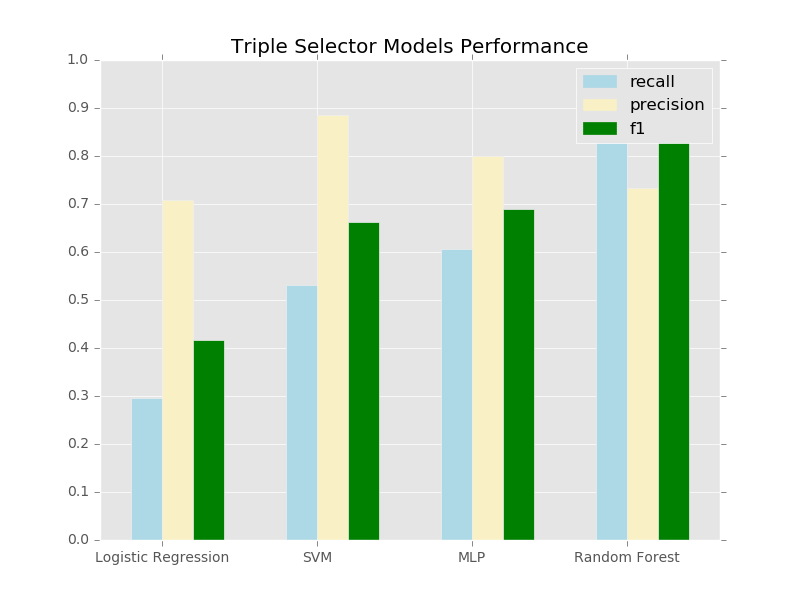
\includegraphics[width=\textwidth]{../images/models_performance_training.png}
	\caption{Diagram hasil eksperimen perbandingan model \textit{supervised learning} untuk \textit{triple selector} dengan menggunakan data latih sebagai data uji}
	\label{fig:models_performance_training}
\end{figure}

\begin{table}
\caption{Hasil eksperimen perbandingan model \textit{supervised learning} untuk \textit{triple selector} dengan menggunakan data latih sebagai data uji}
	\label{tab:models_performance_training}
	\centering
	\begin{tabular}{p{5cm} >{\centering\arraybackslash}p{2cm} >{\centering\arraybackslash}p{2cm} >{\centering\arraybackslash}p{2cm}}
		\hline
		\textbf{Model} & \textbf{\textit{Precision}} & \textbf{\textit{Recall}} & \textbf{$F_1$} \\
		\hline
		Logistic Regression & 0.70 & 0.29 & 0.41 \\
		SVM & \textbf{0.88} & 0.53 & 0.66 \\
		MLP & 0.80 & 0.60 & 0.68 \\
		Random Forest & 0.73 & \textbf{0.96} & \textbf{0.83} \\
		\hline
	\end{tabular}
\end{table}

Selain disebabkan oleh kurangnya jumlah kalimat yang dianotasi, permasalahan pada \textit{dataset} \textit{triple selector} ini juga tentu dipengaruhi oleh kemampuan \textit{triple candidate generator} untuk menghasilkan jumlah kandidat \textit{triple} valid (data positif) yang sebanding jumlahnya dengan kandidat yang tidak valid (data negatif). \saya~berpendapat bahwa, selain menambah data, ada minimal dua solusi yang dapat dilakukan untuk meningkatkan kualitas \textit{dataset}, yaitu:

\begin{enumerate}
	\item Mengekstrak \textit{triple} implisit dari kalimat \\
	Module \textit{triple candidate generator} pada penelitian ini baru menangani \textit{triple} yang memiliki struktur yang eksplisit sehingga jumlah data positif sangat sedikit. Dengan menambah pola \textit{triple} yang dapat dibangkitkan, \textit{dataset} akan lebih seimbang dan memiliki pola lebih banyak \citep{schmitz2012open}. Contoh \textit{triple} eksplisit yang perlu ditangani lebih jauh:
	\begin{itemize}
		\item \textit{Triple} \textit{(kecamatan Kejajar, terletak di, Jawa Tengah)} dari kalimat asal "\textit{Sembungan adalah sebuah desa yang terletak di kecamatan Kejajar, kabupaten Wonosobo, Jawa Tengah, Indonesia.}"		
		\item \textit{Triple} \textit{(Sukarno, adalah, Presiden)} dari kalimat asal "\textit{Presiden pertama Indonesia Sukarno lahir di Surabaya.}"
	\end{itemize} 
	
	\item Mengurangi ekstraksi \textit{triple} invalid dari kalimat \\
	Rasio perbandingan data positif dan negatif pada \textit{dataset} adalah 1:11. Hal ini menunjukkan bahwa proses pembangkitan kandidat \textit{triple} ini masih bisa dibuat lebih efisien. Salah satu teknik yang bisa digunakan adalah membuat aturan yang lebih spesifik atau melatih \textit{classifier} untuk mengekstrak frase \textit{self-contained} \citep{angeli2015leveraging}.
	
\end{enumerate}

Hal menarik yang ditemukan dari hasil eksperimen pertama adalah \textit{random forest}, yang mewakili \textit{ensemble classifier}, merupakan pemodelan yang paling cocok dibandingkan pemodelan linier (\textit{logistic regression}), nonlinier dengan optimalisasi margin (SVM) dan jaringan syaraf tiruan (MLP). \saya~menyimpulkan bahwa dibutuhkan pemodelan yang keseimbangan antara \textit{precision} dan \textit{recall}-nya relatif mudah disesuaikan untuk module \textit{triple selector}. Sekalipun tidak memiliki \textit{precision} setinggi SVM, \textit{Random forest} lebih unggul karena penyesuaian jumlah dan kedalaman \textit{tree} memudahkan penyeimbangan \textit{precision} dan \textit{recall} yang menghasilkan $F_1$ yang paling baik. Potensi SVM yang mampu mencapai \textit{precision} yang paling tinggi ini juga mungkin bisa dimanfaatkan dengan melakukan \textit{bagging} \citep{breiman1996bagging} SVM dan \textit{random forest} untuk meningkatkan kinerja lebih jauh.

Hasil eksperimen kedua menunjukkan bahwa waktu rata-rata ekstraksi per kalimat dari dokumen yang berukuran 5,000 kalimat, 0.002 detik/kalimat, terlihat lebih cepat dari \textsc{TextRunner} yang membutuhkan 0.036 detik/kalimat \citep{banko2007open}. Sekalipun sistem ini tidak bisa diklaim lebih cepat karena adanya perbedaan data uji dan sistem yang digunakan, hasil ini tetap menunjukkan bahwa penggunaan fitur \textit{heavy linguistic} ternyata cukup efisien untuk digunakan pada dokumen dengan ukuran 5,000 kalimat. Trend dari grafik rata-rata waktu proses pada Gambar \ref{fig:system_performance} juga mengindikasikan bahwa sistem akan tetap atau bahkan semakin efisien untuk ukuran dokumen yang lebih besar. 

Grafik rata-rata jumlah \textit{triple} yang diekstraksi per kalimat pada Gambar \ref{fig:system_performance} juga menunjukkan nilai yang cukup konstan pada rentang 2.58-3.12 \textit{triple}/kalimat. Hal ini menunjukkan bahwa sistem berfungsi normal karena seharusnya jumlah \textit{triple} yang dihasilkan per kalimat tidak dipengaruhi oleh ukuran dokumen. Selain itu rata-rata jumlah \textit{triple} yang dihasilkan sistem ini juga sebanding dengan \textsc{TextRunner} yang rata-rata menghasilkan 2.2 \textit{triple}/kalimat \citep{banko2007open}.
